\documentclass[12pt]{article}

% Layout.
\usepackage[top=1in, bottom=0.75in, left=1in, right=1in, headheight=1in, headsep=6pt]{geometry}

% Fonts.
\usepackage{mathptmx}
\usepackage[scaled=0.86]{helvet}
\renewcommand{\emph}[1]{\textsf{\textbf{#1}}}

% TiKZ.
\usepackage{tikz, pgfplots}
\usetikzlibrary{calc}
\pgfplotsset{compat = newest}
\pgfplotsset{my style/.append style={axis x line=middle, axis y line=
middle, xlabel={$x$}, ylabel={$y$}, axis equal }}

% Misc packages.
\usepackage{amsmath,amssymb,latexsym}
\usepackage{graphicx}
\usepackage{array}
\usepackage{xcolor}
\usepackage{multicol}
\usepackage{enumerate}

% Commands to set various header/footer components.
\makeatletter
\def\doctitle#1{\gdef\@doctitle{#1}}
\doctitle{Use {\tt\textbackslash doctitle\{MY LABEL\}}.}
\def\docdate#1{\gdef\@docdate{#1}}
\docdate{Use {\tt\textbackslash docdate\{MY DATE\}}.}
\def\doccourse#1{\gdef\@doccourse{#1}}
\let\@doccourse\@empty
\def\docscoring#1{\gdef\@docscoring{#1}}
\let\@docscoring\@empty
\def\docversion#1{\gdef\@docversion{#1}}
\let\@docversion\@empty
\makeatother

% Headers and footers layout.
\makeatletter
\usepackage{fancyhdr}
\pagestyle{fancy}
\fancyhf{}
\lhead{\baselineskip 30pt
\emph{\@docdate\hfill\@doctitle}
\ifnum \value{page} > 1\relax\else\\
\emph{Name: \rule{3.5in}{1pt}\hfill \@docscoring}\fi}
\rfoot{\emph{\@docversion}}
\lfoot{\emph{\@doccourse}}
\cfoot{\emph{\thepage}}
\renewcommand{\headrulewidth}{0pt}
\makeatother

% Paragraph spacing
\parindent 0pt
\parskip 6pt plus 1pt

% Problem counters
\newcounter{probcount}
\newcounter{subprobcount}
\setcounter{probcount}{0}

\newcommand{\problem}[1]{%
\par\addvspace{4pt}%
\setcounter{subprobcount}{0}%
\stepcounter{probcount}%
\makebox[0pt][r]{\emph{\arabic{probcount}.}\hskip1ex}\emph{[#1 points]}\hskip1ex}

\newenvironment{subproblems}{%
\begin{enumerate}%
\setcounter{enumi}{\value{subprobcount}}%
\renewcommand{\theenumi}{\emph{\alph{enumi}}}}%
{\setcounter{subprobcount}{\value{enumi}}\end{enumerate}}

% Blanks
\newcommand{\blank}[1]{\rule{#1}{0.5pt}}
\newcommand{\mblank}[1]{\underline{\hspace{#1}}}

% Display helpers
\renewcommand{\d}{\displaystyle}
\newcommand{\ds}{\displaystyle}

% Document info
\doctitle{Math F251X: Quiz 3}
\docdate{January 29, 2026}
\doccourse{UAF Calculus I}
\docversion{Spring 2026}
\docscoring{\blank{0.8in} / 25}

\begin{document}

\emph{Please circle your instructor's name:}
\hfill James Gossell \hfill Gordon Williams \\

There are 25 points possible on this quiz.
Any outside materials are not allowed.
\emph{For full credit, show all work clearly.}

%------------------------------------------------
\problem{10}
Use the graph of the function $f(x)$ to answer each question. If the limit is infinite, indicate that with $\infty$ or $-\infty$. If the value does not exist or is undefined, write DNE.

\begin{center}
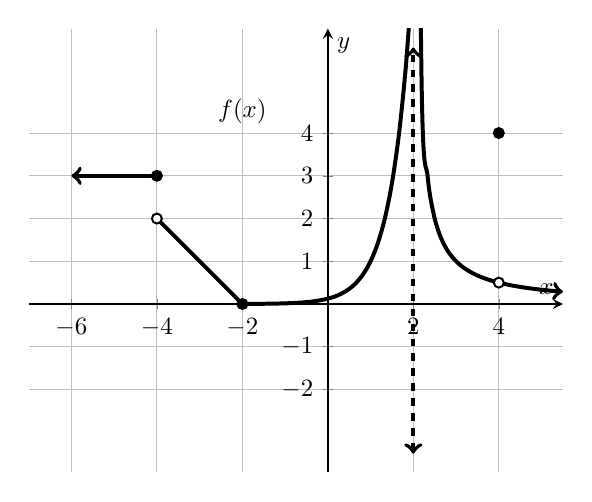
\begin{tikzpicture}[scale=0.9]
\begin{axis}[scale=1.1, thick, my style,
xmin=-7, xmax=5.5,
ymin=-2.5, ymax=5,
xtick={-6,-4,-2,0,2,4},
ytick={-2,-1,1,2,3,4},
grid=both]

% Vertical asymptote
\addplot[dashed,<->, ultra thick] coordinates {(2,-3.5) (2,6)};

% Left horizontal piece
\addplot[ultra thick, <-] coordinates {(-6,3)(-4,3)};

% Linear piece from -4 to -2
\addplot[ultra thick] coordinates {(-4,2)(-2,0)};

% Exponential piece: 8^(x-1) for -2 <= x <= 2
\addplot[ultra thick, smooth, domain=-2:2] {8^(x-1)};

% Rational piece: 1/(x-2) for x > 2 (with arrow)
\addplot[ultra thick, smooth, ->, domain=2.05:5.5] {1/(x-2)};

% Filled points
\addplot[mark=*, only marks] coordinates {(-4,3) (-2,0) (4,4)};

% Open point
\addplot[mark=*, fill=white, only marks] coordinates {(-4,2) (4,0.5)};

\node at (-2,4.5) {$f(x)$};
\end{axis}
\end{tikzpicture}
\end{center}

\begin{subproblems}
\begin{multicols}{3}
\item $\d \lim_{x \to -4^-} f(x) = \mblank{.5in}$
\item $\d \lim_{x \to -4^+} f(x) = \mblank{.5in}$
\item $\d \lim_{x \to -4} f(x) = \mblank{.5in}$
\end{multicols}

\begin{multicols}{3}
\item $\d \lim_{x \to 2^+} f(x) = \mblank{.5in}$
\item $\d f(4) = \mblank{.5in}$
\item $\d \lim_{x \to 4} f(x) = \mblank{.5in}$
\end{multicols}

\item Write the domain of $f(x)$: \blank{3in}

\item List all $x$-values for which $f(x)$ is {\bf not} continuous. For each of your answers, classify the discontinuity as {\bf jump}, {\bf removable}, {\bf infinite}, or {\bf other}.\\



\blank{6in}

\vspace{.2in}

\problem{5} Determine whether the given function is continuous at $x=0$. Justify your answer {\bf using limits}.
\[
g(x)=
\begin{cases}
x^2 - e^x, & x < 0 \\[6pt]
1-x, & x \ge 0
\end{cases}
\]

\end{subproblems}

%------------------------------------------------
\newpage

\problem{8}
Evaluate the limits algebraically. Show all work.

\begin{subproblems}
\item $\d \lim_{x \to 3} \frac{x^2-x-6}{12-4x} =$
\vfill
\item $\d \lim_{x \to 4} \frac{3x-12}{\sqrt{x}-2} =$
\vfill
\end{subproblems}




%------------------------------------------------
\problem{2}

Evaluate the limit below.  
\textbf{Circle one answer from Part I and one justification from Part II.}

\[
\lim_{x \to 3^-} \frac{2x-7}{x^2-9}
\]

\medskip

\textbf{Value of the Limit (Circle one)}

\begin{center}

{\Large $\displaystyle -\infty$ \hspace{3cm} $\displaystyle +\infty$ \hspace{3cm} $\displaystyle 0$}

\end{center}

\medskip

\textbf{Justification (Circle one)} As $x$ approaches $3$ from the left...

\begin{enumerate}[(A)]
\item ...the numerator is positive and the denominator is slightly bigger than $0$.
\item ...the numerator is positive and the denominator is slightly smaller than $0$.
\item ...the numerator is negative and the denominator is slightly bigger than $0$.
\item ...the numerator is negative and the denominator is slightly smaller than $0$.
\item ...the limit is $0$ because the denominator is equal to $0$.
\end{enumerate}



\end{document}